\chapter{Analiza FLUENT - rețele profile separate}\label{chapter:analiza}

Pentru a ne asigura că rezultatele obținute cu ajutorul calculelor proprii și cu ajutorul codului dezvoltat "in-house" de catedra de Mașini Hidraulice din Timișoara, dorim sa verificam rezultatele într-un software profesional dezvoltat pentru acest fel de aplicații și anume Ansys FLUENT.

Analizăm așadar rezultatele obținute prin optimizare numerică și prin analiza în FLUENT pentru coeficientul de presiune pe cele doua profile separate.

\section{Rețele profile separate. Stator}

\begin{figure}[h]
	\centering
	\includegraphics[scale=0.5]{figures/cp-stator-ezdraw.eps}
	\caption{Coeficient de presiune stator - optimizare numerică / analiză FLUENT}
	\label{Coeficient de presiune stator - optimizare numerică / analiză FLUENT}
\end{figure}

\clearpage



\section{Rețele profile separate. Rotor}

\begin{figure}[h]
	\centering
	\includegraphics[scale=0.5]{figures/cp-rotor-ezdraw.eps}
	\caption{Coeficient de presiune rotor - optimizare numerică / analiză FLUENT}
	\label{Coeficient de presiune rotor - optimizare numerică / analiză FLUENT}
\end{figure}

Se poate observa că valorile obținute prin cele două metode sunt extrem de apropiate, lucru care ne validează rezultatele cu un anumit grad de siguranță, fără sa avem la îndemâna o validare experimentala.

\clearpage


\section{Reprezentare analiză în tandem din FLUENT}

\begin{figure}[h]
	\centering
	\includegraphics[scale=0.5]{figures/AXENT-tandem-streamlines-ezdraw.eps}
	\caption{Reprezentare linii de curent în tandemul stator-rotor pentru turbina AXENT / analiză FLUENT}
	\label{Reprezentare linii de curent în tandemul stator-rotor pentru turbina AXENT / analiză FLUENT}
\end{figure}

Cu ajutorul FLUENT putem simula și în tandem cele doua rețele de profile, pentru a avea o imagine mai bună asupra fenomenelor hidrodinamice care apar în turbină. În figura 4.3 se pot observa liniile de curent peste cele două profile precum și triunghiurile de viteze calculate inițial.

\clearpage